\section{影响 MAS 性能因素的补充讨论}
\label{ap:discuss_control}


\subsection{鲁棒性维度上的 MAS 与 SAS 对比}
\label{ap:mas_sas_robustness}


\begin{center}
\vspace{-0.5\baselineskip}
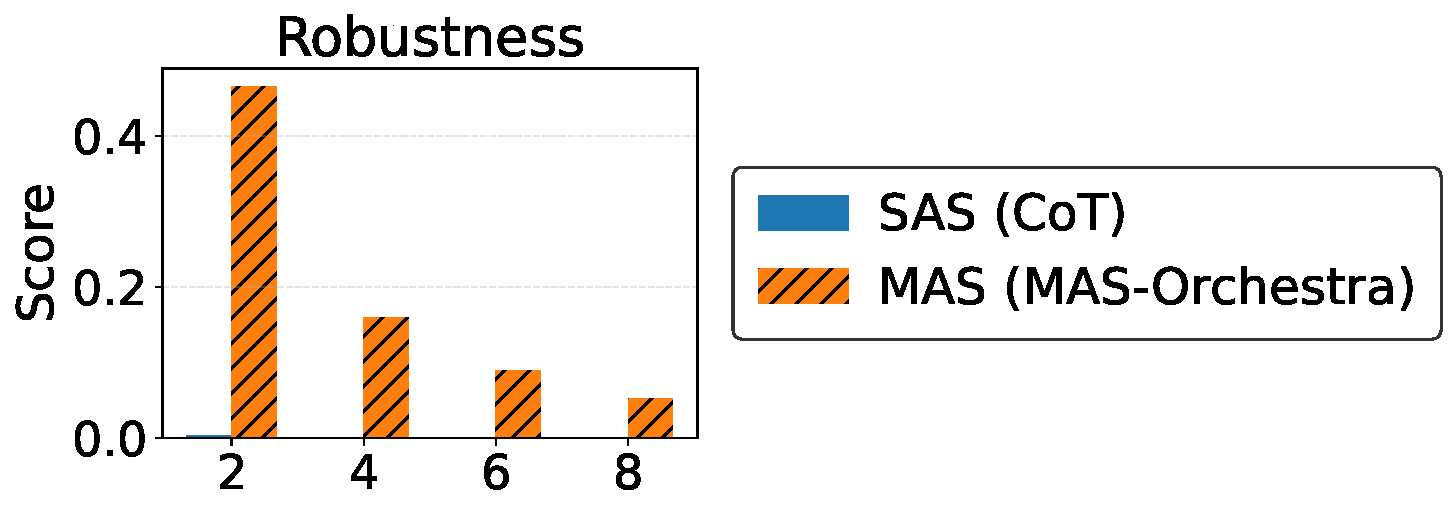
\includegraphics[width=0.5\columnwidth]{figs/oss120b_robustness.pdf}
\vspace{-0.5\baselineskip}
\captionof{figure}{\small 使用 \ossonetwentylow 作为子智能体时，\robustness{}设置下的 \avgat{8}。（SAS 性能过低，图中不可见。）}
% \zixuan{TODO: update the bg color}
\label{fig:robustness}
\end{center}



在\cref{tab:sas_mas_example}中，我们展示了一个来自\robustness{}维度（\robustness{}等于 2）的样本，其中编排器为 \qwen，子智能体为 \ossonetwenty（SAS 情况下即为主智能体）。详细描述与观察见\cref{sec:subtask_structure}。

\begin{table*}[h]
\centering
\small
% \addtolength{\tabcolsep}{-0.4em}
\begin{tabularx}{\textwidth}{l X X}
\toprule
 & \textbf{单智能体系统（SAS）} & \textbf{多智能体系统（MAS）} \\
\midrule
\textbf{问题}
& \multicolumn{2}{p{0.76\linewidth}}{
从段落中识别并返回：（1）thundering-autumn 的魔法数字；（2）Beach Backpack 拥有的 Accordion File 数量。每项使用 \texttt{\textbackslash boxed\{\}} 包裹，并用两个换行符分隔。
} \\
\midrule
\textbf{思考过程}
&
我们从注释中识别出魔法数字为 7381734。
Insulated Backpack 的 Accordion File 数量为 21，而 Beach Backpack 的 Accordion File 数量是它的两倍，因此为 42。
答案由两个带方框的数字组成，并以两个换行符分隔。
&
任务被分解为两个子问题：
（1）从段落中提取 thundering-autumn 的魔法数字；
（2）利用给定关系计算 Beach Backpack 拥有的 Accordion File 数量。
由一个汇点智能体格式化最终输出。
\\
\midrule
\textbf{MAS 设计}
&
不适用
&
\hspace{-50mm}
\raisebox{-0.5\height}{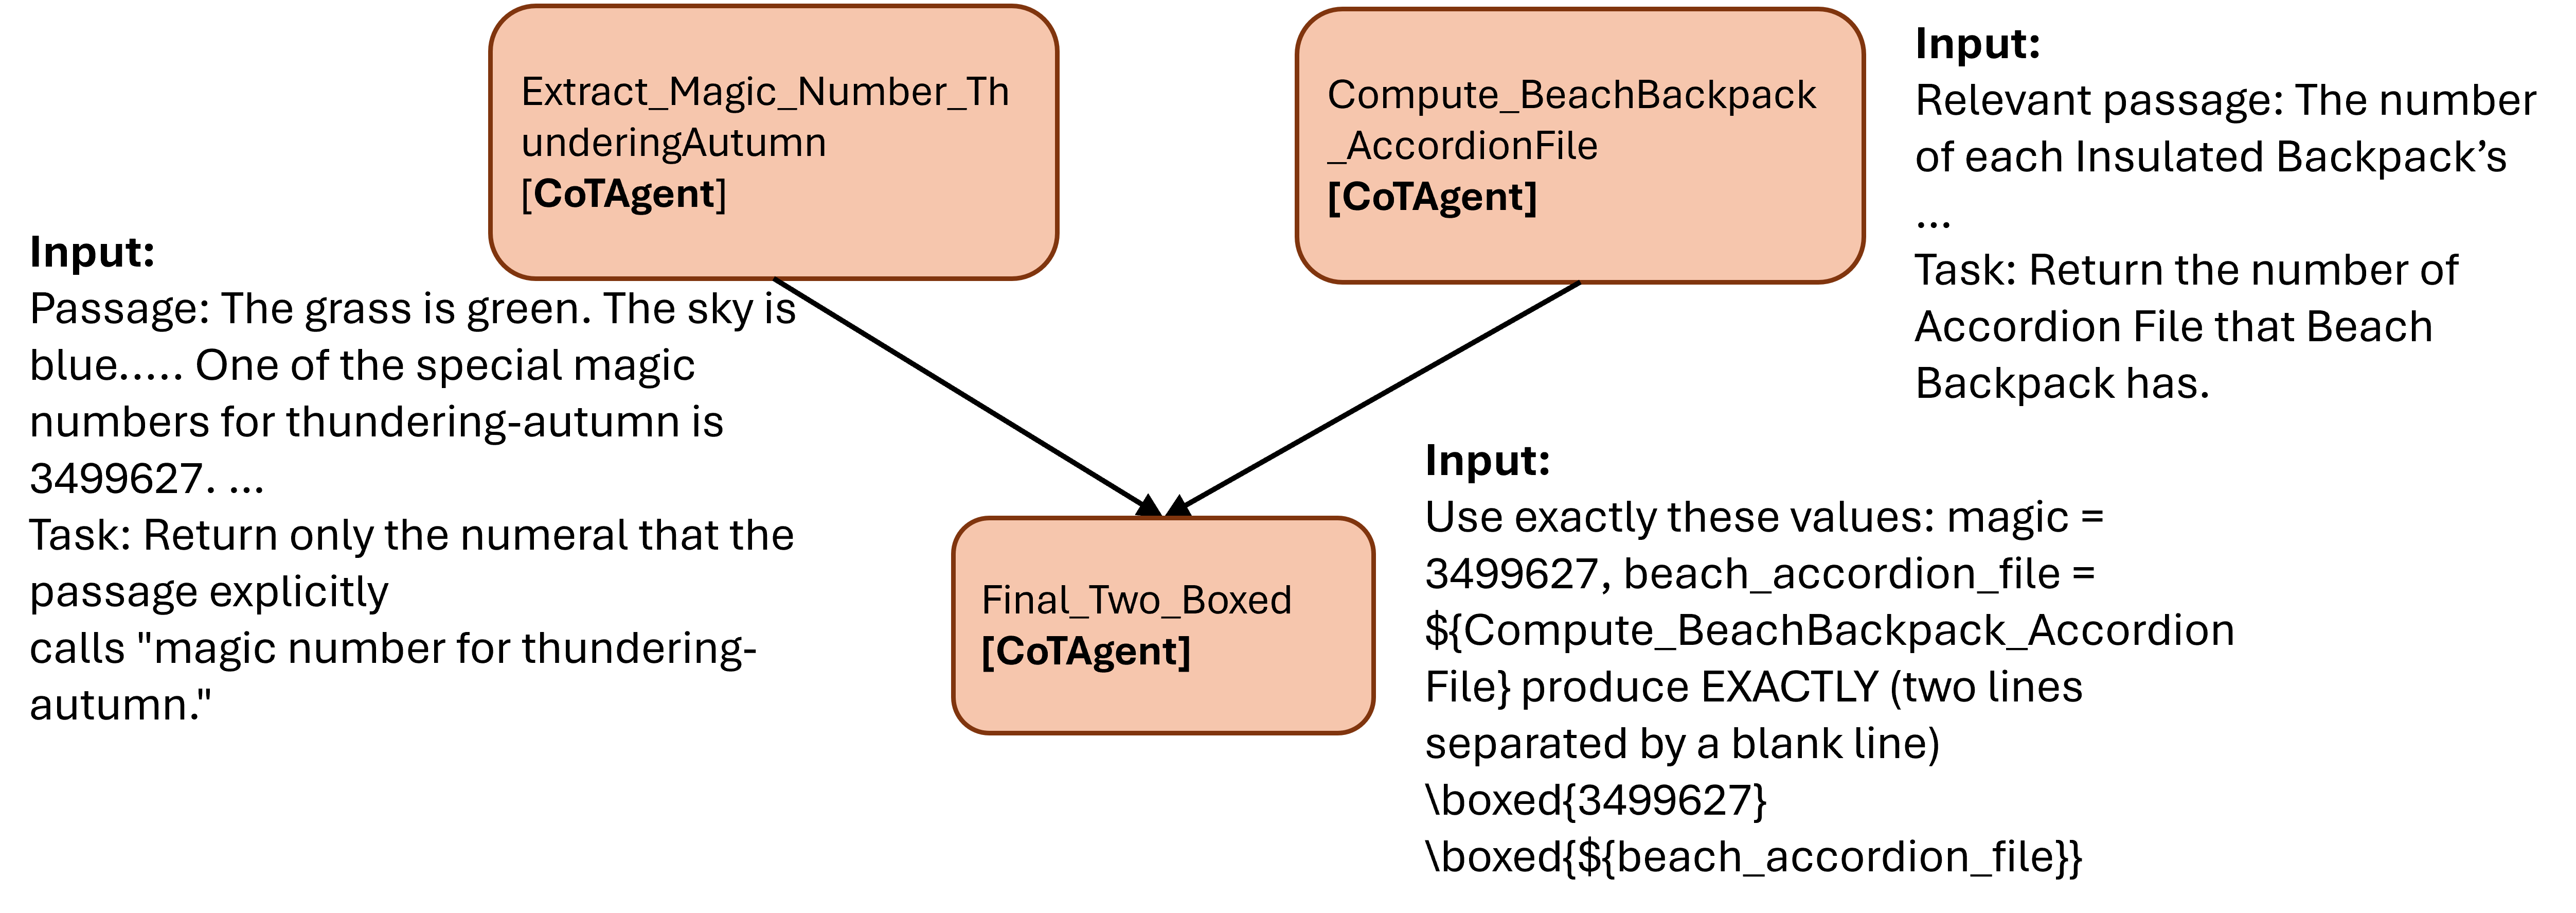
\includegraphics[height=4.1cm]{figs/sas_vs_mas.png}}
\\
\midrule
\textbf{执行输出}
&
\boxed{7381734}

\boxed{42}
&
\boxed{3499627}  

\boxed{19}
\\
\midrule
\textbf{真实答案}
& \multicolumn{2}{c}{
\boxed{3499627} \boxed{19}
} \\
\bottomrule
\end{tabularx}
\caption{单智能体系统（SAS）与多智能体系统（MAS）在同一问题实例上的对比。
% \zixuan{where is this sample from}
}
% from https://vincent950129.github.io/mas-design/mas_r1/qwen2.5_7b_oss_120b_low_conflict2.html and call GPT-OSS at real time
\label{tab:sas_mas_example}
\end{table*}


% \zixuan{working}
\subsection{鲁棒性与对抗感知训练}需要特别指出的是，\cref{fig:mas_combined_comparison}中\robustness{}维度的结果来自包含对抗样本的混合训练数据。然而在实践中，这类样本往往不可得或被省略。为研究这一影响，\cref{fig:robustness_combine}比较了在包含和不包含对抗样本的混合数据上训练的模型。我们观察到，排除对抗数据后，\robustness{}维度的性能仍然很差，几乎为零，与\cref{fig:robustness}中的 SAS 性能相当。这一结果表明，尽管混合训练能在多数维度上良好泛化，却无法泛化到鲁棒性。因此，要提升鲁棒性性能，必须显式加入对抗数据。


\textbf{说明。}分开训练与混合训练需要不同数量的训练步骤，因为混合数据集自然更大。我们的实验目标并非让强化学习训练完全收敛，而是考察不同因素如何影响 MAS 性能。在实验中，混合训练使用的训练步骤数是分开训练的两倍。我们预计，增加训练步骤还能进一步提升混合训练的性能。


%%%%%%%%%%%%%%%%%%%%%%%%%%%%%%

\subsection{所有维度的智能体统计}

\cref{fig:axes_detail}给出了不同评估维度（\depth、\horizon、\breadth、\myparallel{}和\robustness）下生成的子智能体总数统计。结果表明，编排器基本能够学会在编排设计中映射底层任务结构。然而，如前文所述，这种结构对齐并不一定会转化为相对于 SAS 的性能收益。

% \cref{fig:axes_detail} shows detailed statistics of the total number of sub-agents generated under different evaluation axes (\depth, \horizon, \breadth, \myparallel, and \robustness), using \qwen as the orchestrator and \ossonetwenty as the sub-agent.

\begin{figure*}[h!]
\centering
% \vspace{-2\baselineskip}
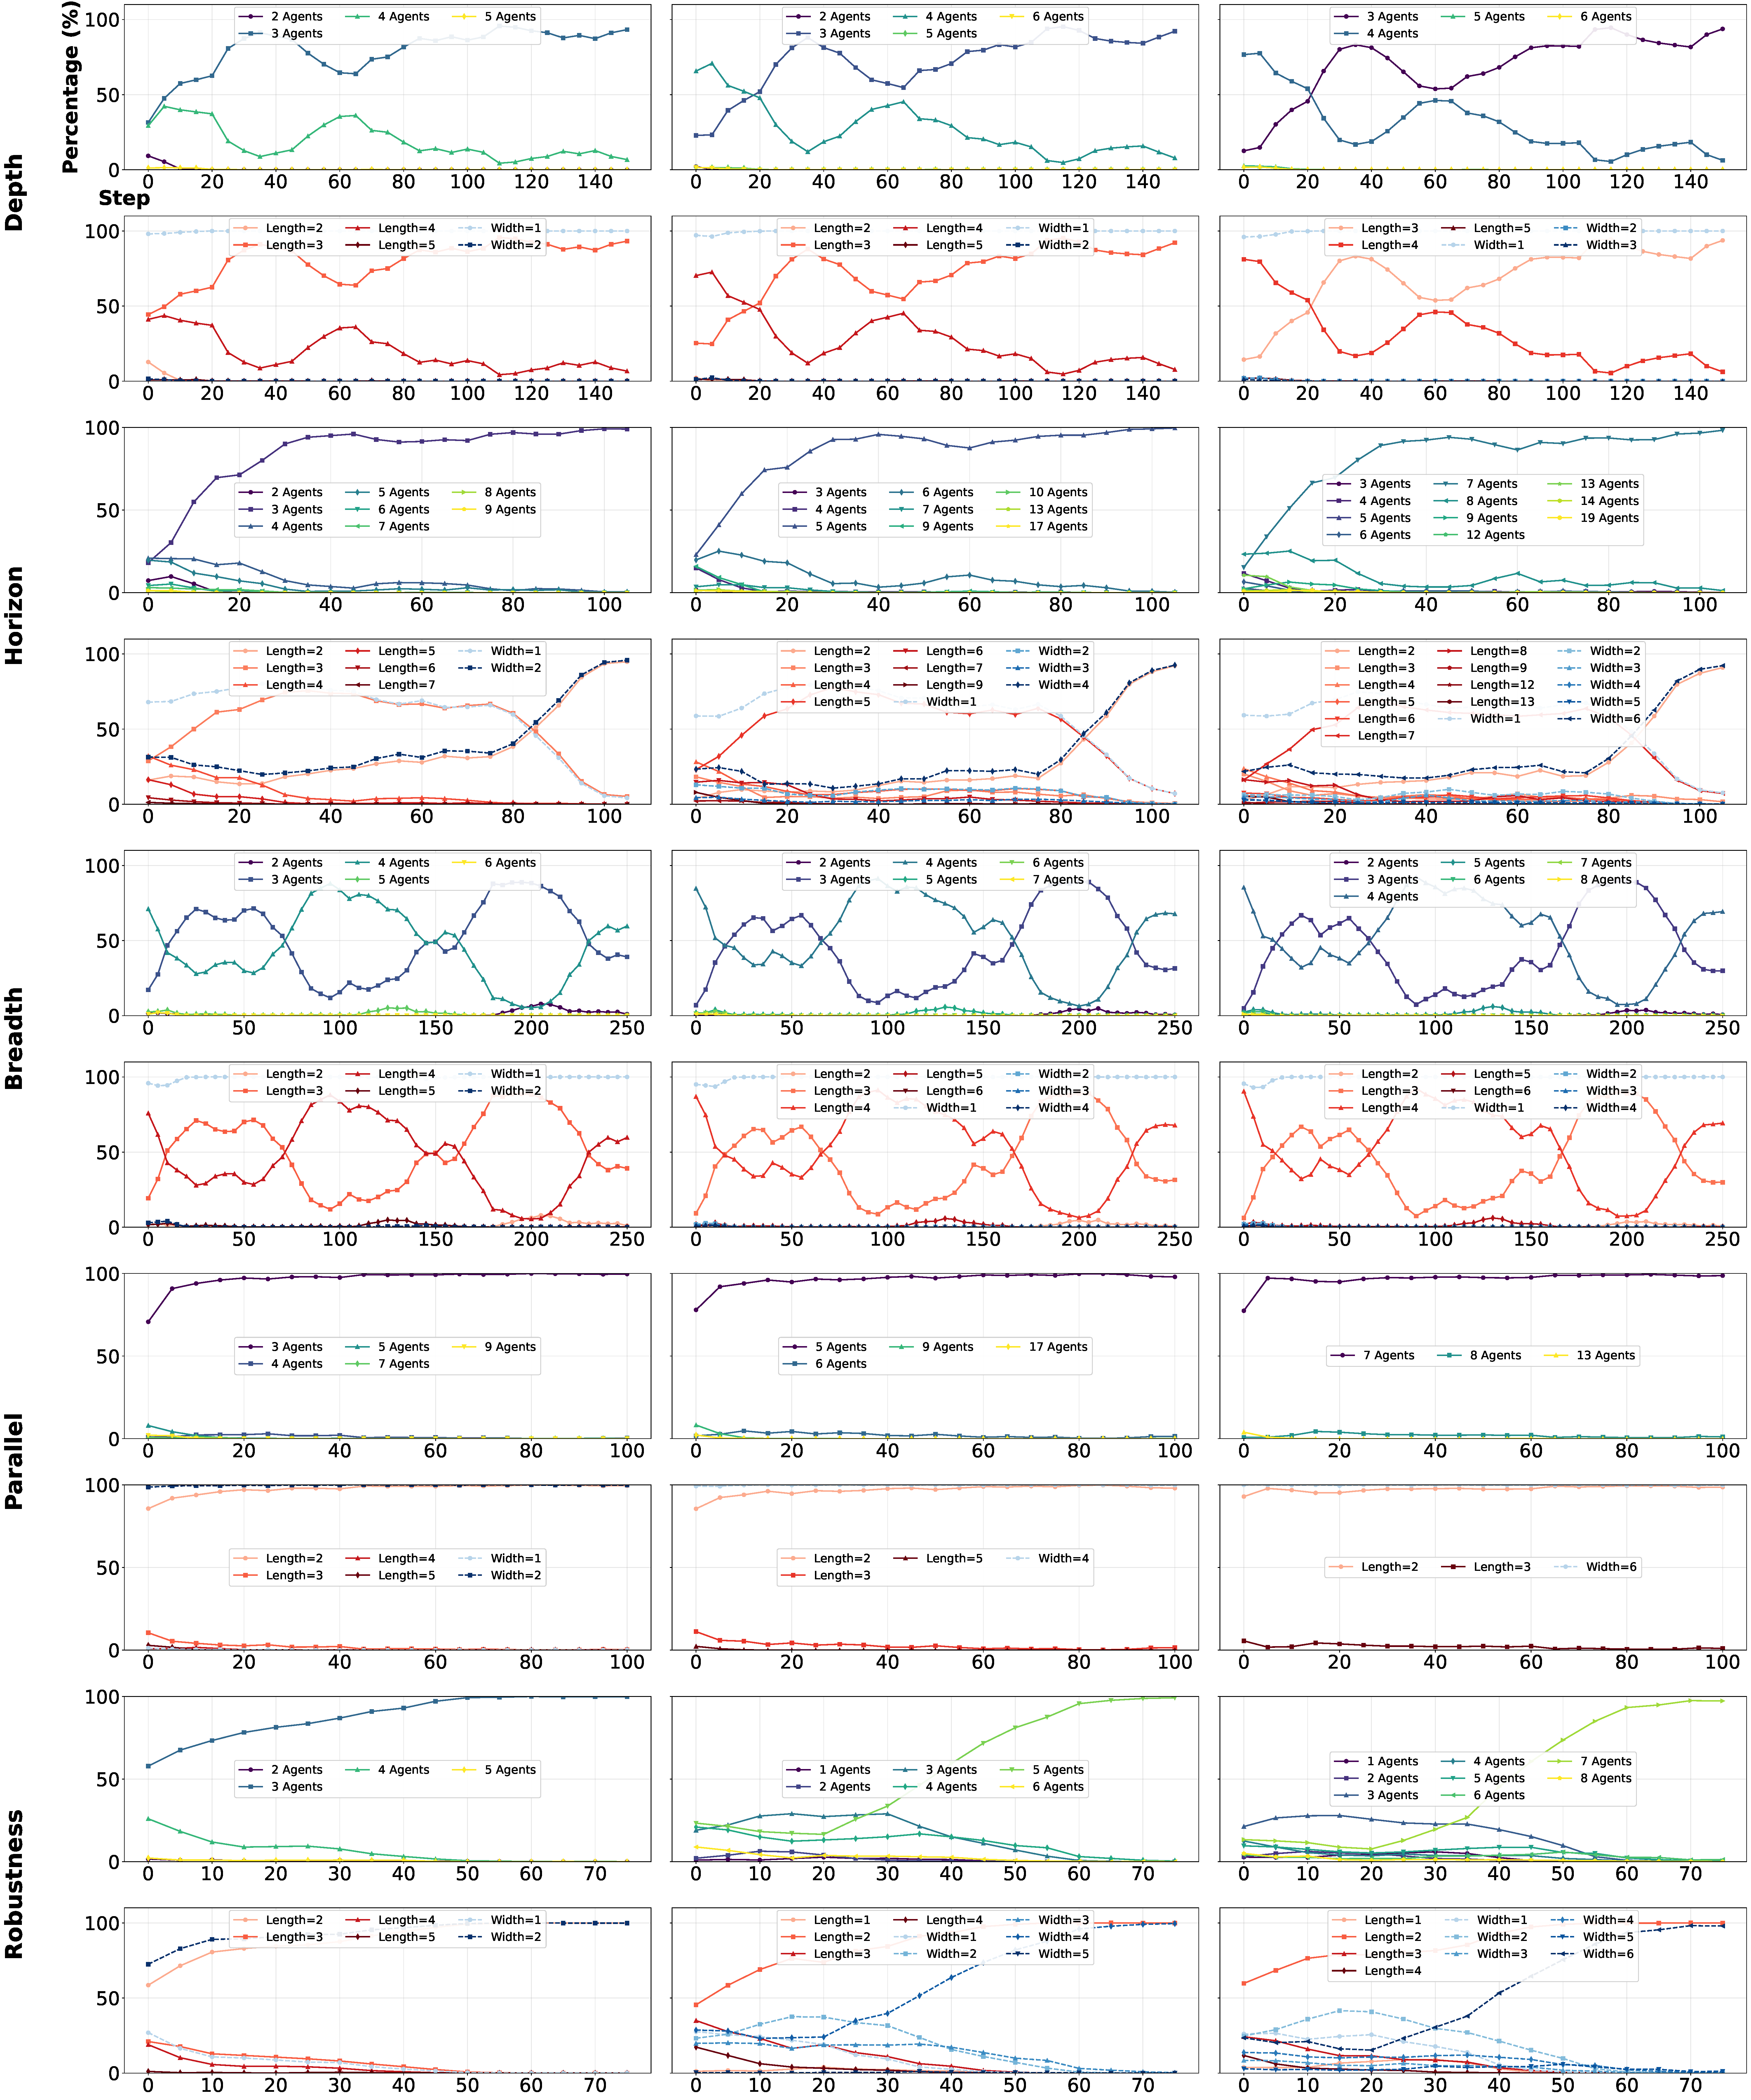
\includegraphics[width=\columnwidth]{figs/7b_120b_low_combine.pdf}
\vspace{-\baselineskip}
\captionof{figure}{\small 不同维度的智能体统计（从左到右对应取值 2、4、6）。}
\label{fig:axes_detail}
\end{figure*}

% As discussed in \cref{sec:subtask_structure}, overall, these results show that the orchestrator can largely learn to mirror the underlying task structure in its orchestration design. 

下面给出几项详细观察。

\subsubsection{固定维度时不同取值间的观察}

我们首先考察固定维度内部的结果。随着任务复杂度增加（即维度取值增大），系统会\textbf{生成更多子智能体}。这一行为符合预期，说明编排器能够有效适应不断增长的任务复杂度。

我们还观察到，在同一维度内，尽管子智能体数量有所增加，不同取值下的整体编排模式仍然相似。这说明编排器学习到的结构策略具有\textbf{稳定性}：随着任务复杂度增长，它会扩展子智能体数量，但不会改变底层编排结构。

% whereas \myparallel and \horizon exhibit more diverse multi-agent structures.

% We observed that \depth and \breadth tends converg to a general sequential (i.e., \text{Parse → Solve → Verify → Final Answer}), while \myparallel parallel MAS and Horizon is relatively more diverse.


% MAS Pattern: Depth and Breadth converged to a general sequential (Parse → Solve → Verify → Final Answer). Parallel converges to parallel MAS and Horizon is relatively more diverse.

\subsubsection{固定取值时不同维度间的观察}

我们观察到，\depth{}和\breadth{}往往收敛到一种通用的顺序模式。具体而言，长度通常为 1 到 5，而宽度要小得多，一般不超过 2。进一步检查生成样本可以发现，所得 MAS 通常遵循“\text{解析} $\rightarrow$ \text{求解} $\rightarrow$ \text{验证} $\rightarrow$ \text{最终答案}”结构。这表明，对于具有顺序依赖链或扇入结构的任务，在当前设置下，包含显式中间推理的线性分解已经足够且稳定。

相比之下，\myparallel{}往往收敛到并行 MAS 结构，其宽度通常与指定的\myparallel{}取值一致。这种行为紧密映射了底层任务结构，说明在当前训练方法下，编排器能有效学习并利用相互独立的子任务结构。

对于\horizon，观察到的结构多样性反映了“何时应显式给出中间结果”这一问题的不确定性。部分任务受益于较早合成局部答案，另一些任务则需要在若干推理步骤后延迟聚合。编排器会针对不同时域设置改变子智能体数量与顺序，这说明 \ourframework 从任务级反馈中学习时间控制策略，而非依赖固定的推理深度。

对于\robustness，我们观察到系统倾向于采用并行 MAS 结构。这种编排策略允许不同子智能体处理不同子任务，并有助于在单个子智能体内部，或借助额外的验证、仲裁组件，隔离并缓解对抗性或错误信息。


% We observe that \depth and \breadth tend to converge to a general sequential pattern (i.e., length ranges from 1 to 5 while the width is much smaller, usualy up to 2. A further look at example can be foudn that the geenrataer MAS is typrcially \text{Parse} $\rightarrow$ \text{Solve} $\rightarrow$ \text{Verify} $\rightarrow$ \text{Final Answer}), indicating that for tasks with long dependency chains or large fan-in, a linear decomposition with explicit intermediate reasoning is both sufficient and stable for the given setting. \myparallel tebnd to converge to parallel MAS (wideht typically the same as the \parallel value), clealry mirror the task structure, indicating that it is suffiicent to learn the indendepcnt t structuire ia current method. In contrast, For \horizon, the observed diversity reflects uncertainty about when intermediate results should be made explicit. Some tasks benefit from early synthesis of partial answers, while others require delayed aggregation after several reasoning steps. The orchestrator adapts by varying both the number and ordering of sub-agents across horizon settings, suggesting that \ourframework learns temporal control strategies based on task feedback rather than relying on a fixed reasoning depth. For \robstuness, we observat that it tend to concerge to parallel MAS, which is a smart orchesttation that can enable diffetnet sub-agent address different sub-task and effeictively handle the adversatial information within individual sub-agent or an additional moderatotrr.

% MAS Pattern: conflict convereges to parallel MAS


% \zixuan{maybe we can use table with figures}

% \begin{table*}[h]
% \centering
% \small
% \setlength{\tabcolsep}{6pt}
% \renewcommand{\arraystretch}{1.05}
% \begin{tabular}{c m{0.27\textwidth} m{0.27\textwidth} m{0.27\textwidth}}
% \toprule
% \textbf{Axis} & \textbf{Value = 2} & \textbf{Value = 4} & \textbf{Value = 6} \\
% \midrule

% Depth &
% \includegraphics[width=\linewidth]{figs/7b_120b_low_individual_depth2.pdf} &
% \includegraphics[width=\linewidth]{figs/7b_120b_low_individual_depth4.pdf} &
% \includegraphics[width=\linewidth]{figs/7b_120b_low_individual_depth6.pdf} \\[-2pt]

% Horizon &
% \includegraphics[width=\linewidth]{figs/7b_120b_low_individual_horizon2.pdf} &
% \includegraphics[width=\linewidth]{figs/7b_120b_low_individual_horizon4.pdf} &
% \includegraphics[width=\linewidth]{figs/7b_120b_low_individual_horizon6.pdf} \\[-2pt]

% Breadth &
% \includegraphics[width=\linewidth]{figs/7b_120b_low_individual_breadth2.pdf} &
% \includegraphics[width=\linewidth]{figs/7b_120b_low_individual_breadth4.pdf} &
% \includegraphics[width=\linewidth]{figs/7b_120b_low_individual_breadth6.pdf} \\[-2pt]

% Parallel &
% \includegraphics[width=\linewidth]{figs/7b_120b_low_individual_parallel2.pdf} &
% \includegraphics[width=\linewidth]{figs/7b_120b_low_individual_parallel4.pdf} &
% \includegraphics[width=\linewidth]{figs/7b_120b_low_individual_parallel6.pdf} \\[-2pt]

% Robustness &
% \includegraphics[width=\linewidth]{figs/7b_120b_low_individual_conflict2.pdf} &
% \includegraphics[width=\linewidth]{figs/7b_120b_low_individual_conflict4.pdf} &
% \includegraphics[width=\linewidth]{figs/7b_120b_low_individual_conflict6.pdf} \\

% \bottomrule
% \end{tabular}
% \end{table*}
% \zixuan{may need to draw a big figure instead, too small}


% \zixuan{TODO: put results for combination training here}


\subsection{分开训练与混合训练}

% \subsection{Separate vs. Combined training.} 
在\cref{fig:sub_task_sub_agent}中，我们使用来自不同维度的训练数据分别训练编排器。现在，我们考察：\textit{能否合并不同维度的数据进行训练，以及由此得到的编排器能否在单独维度的测试中泛化？}\cref{fig:mas_combined_comparison}给出了在全部五个维度的混合数据上训练所得的结果。我们观察到，不同维度上的性能非常相似，说明编排器在混合数据上训练后能够有效泛化。



% In \cref{fig:mas_combined_comparison}, we demonstrate results obtained by training on combined data from all five axes. See \cref{sec:subtask_structure} for detailed descriptions and observation.

% In \cref{fig:sub_task_sub_agent}, we train the orchestrators using training
% data from different axes. Now, we examine: \textbf{can data from different axes be combined for
% training, and can the resulting orchestrator generalize when tested on
% individual axes?} \cref{fig:mas_combined_comparison} reports results obtained by training on
% combined data from all four axes (excluding \robustness). We observe that the
% performance across different axes is highly similar, indicating that the
%  the orchestrator can effectively generalize when
% trained on combined data from multiple axes. 

% \shafiq{If the robustness results reported before and in Fig 4 (without combined) with training on robustness, we need to reorganize this section. Let's talk about this.} \zixuan{TODO: first talk about combine has the same observation as individual, and then discuss that removing robustness data will cause significant degrade on robustness (details move to Appendix \cref{ap:discuss_combine_training} as the observation is similar as individual)}

\begin{center}
\vspace{-0.5\baselineskip}
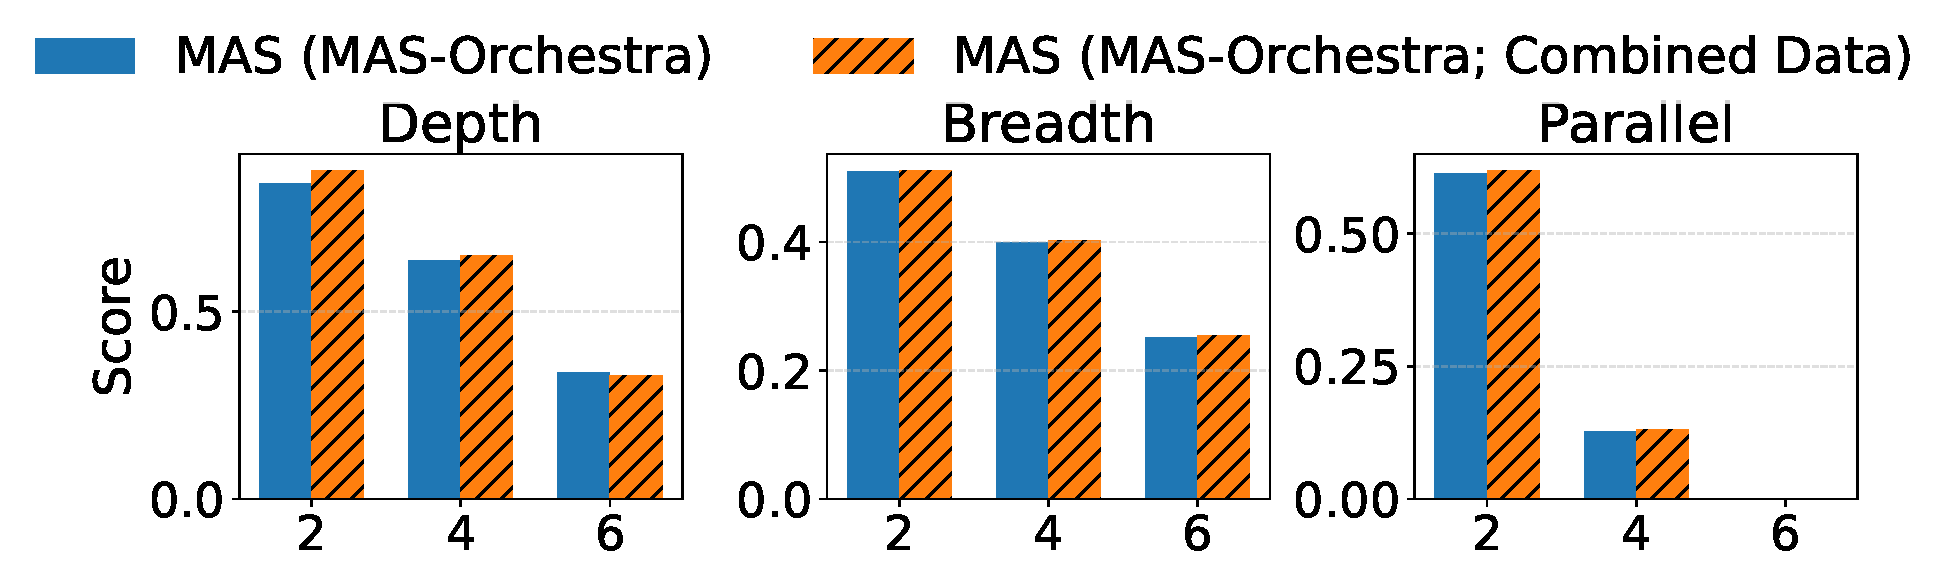
\includegraphics[width=0.6\columnwidth]{figs/mas_combined_comparison.pdf}
\vspace{-10pt}
\captionof{figure}{\small 分开训练与混合训练的 \avgat{8} 对比。
% \shafiq{why there is no horizon?}\zixuan{the combine experiemtns is not as complete as individual, will move to Appendix}\zixuan{still missing at the moment}
}
% \zixuan{TODO: add robustness as well: canot generalize to robustness}
\label{fig:mas_combined_comparison}
\end{center}




\textbf{\robustness。}
% A straightforward way to address the above issue is to incorporate robustness
% training data during training. 
\cref{fig:robustness_combine}比较了在混合数据上训练、但分别包含和不包含对抗样本的模型。我们观察到，加入对抗训练数据后，性能相较不使用此类数据时显著提升。这一结果说明，要提高鲁棒性性能，必须在混合训练数据中显式加入对抗样本。


\begin{center}
% \vspace{-0.5\baselineskip}
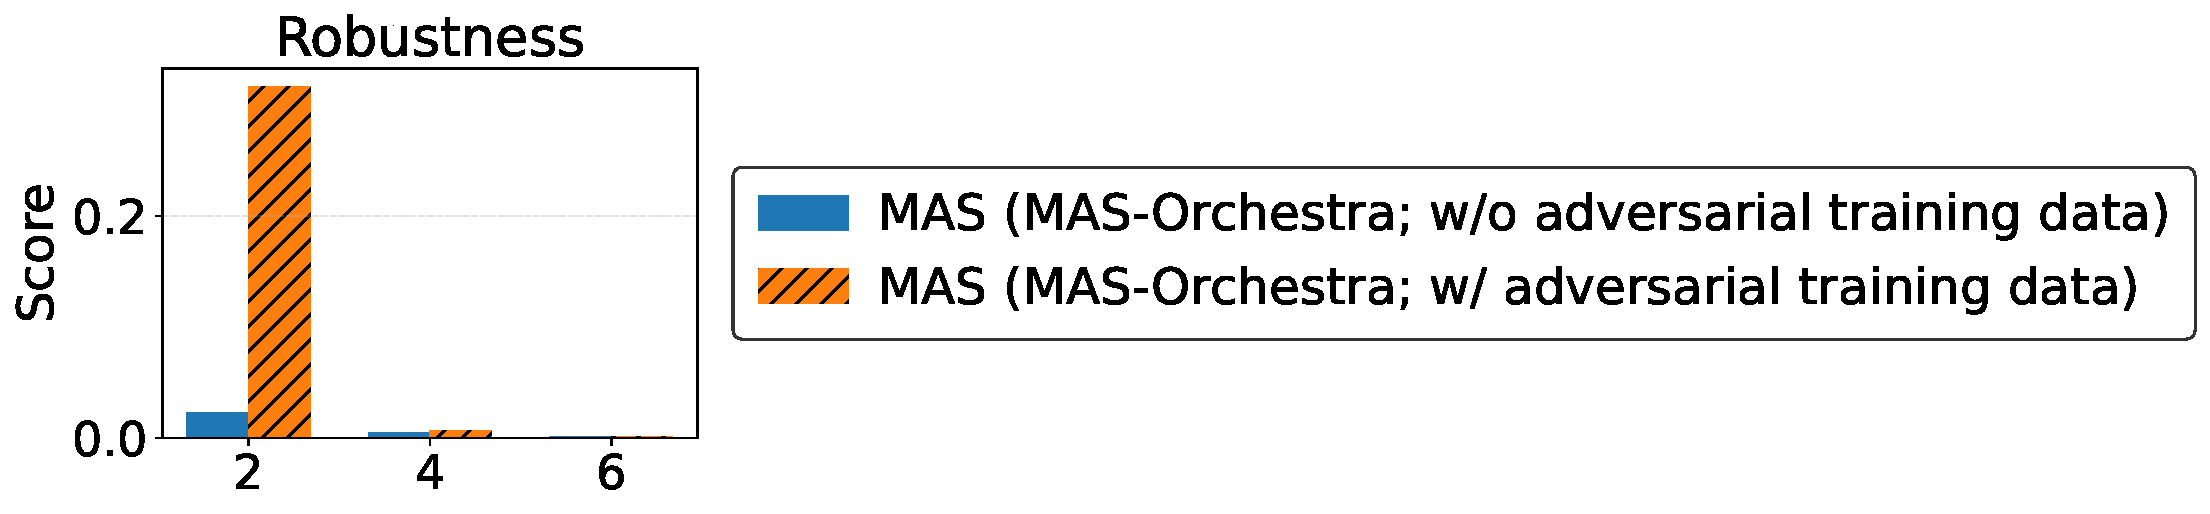
\includegraphics[width=0.6\columnwidth]{figs/oss120b_robustness_combine.pdf}
\vspace{-0.5\baselineskip}
\captionof{figure}{\small 采用和不采用对抗感知训练时，\robustness{}混合训练的 \avgat{8}。}
\label{fig:robustness_combine}
\end{center}

% \shafiq{If we need space, this can go to Appendix with a brief summary in the main body. Let's talk}

% \subsection{Does RLM orchestrator size affect MAS performance?}
\subsection{RLM 编排器规模如何影响 MAS 性能？}

由于 \qwen 是 7B 模型，而前述 RLM 拥有 20B 参数，人们或许会怀疑模型规模是否造成了观察到的性能差距。为此，我们在混合训练下比较 7B RLM DeepSeek-R1-Distill-Qwen-7B（\deepseekqwen）\cite{deepseekai2025deepseekr1incentivizingreasoningcapability}与 \qwen，并使用相近的训练步数。如\cref{fig:deepseek}所示，即使控制模型规模，RLM 在不同维度上仍然始终逊于 LLM。这一结果说明，当前 RLM 并不适合充当编排器。

% \shafiq{If we need space, this can go to Appendix with a brief summary in the main body}

\cref{fig:deepseek}比较了使用同等规模的指令微调 LLM 与 RLM 时的性能，详细说明见\cref{sec:reasoning_meta_agent}。

\begin{center}
\vspace{-0.5\baselineskip}
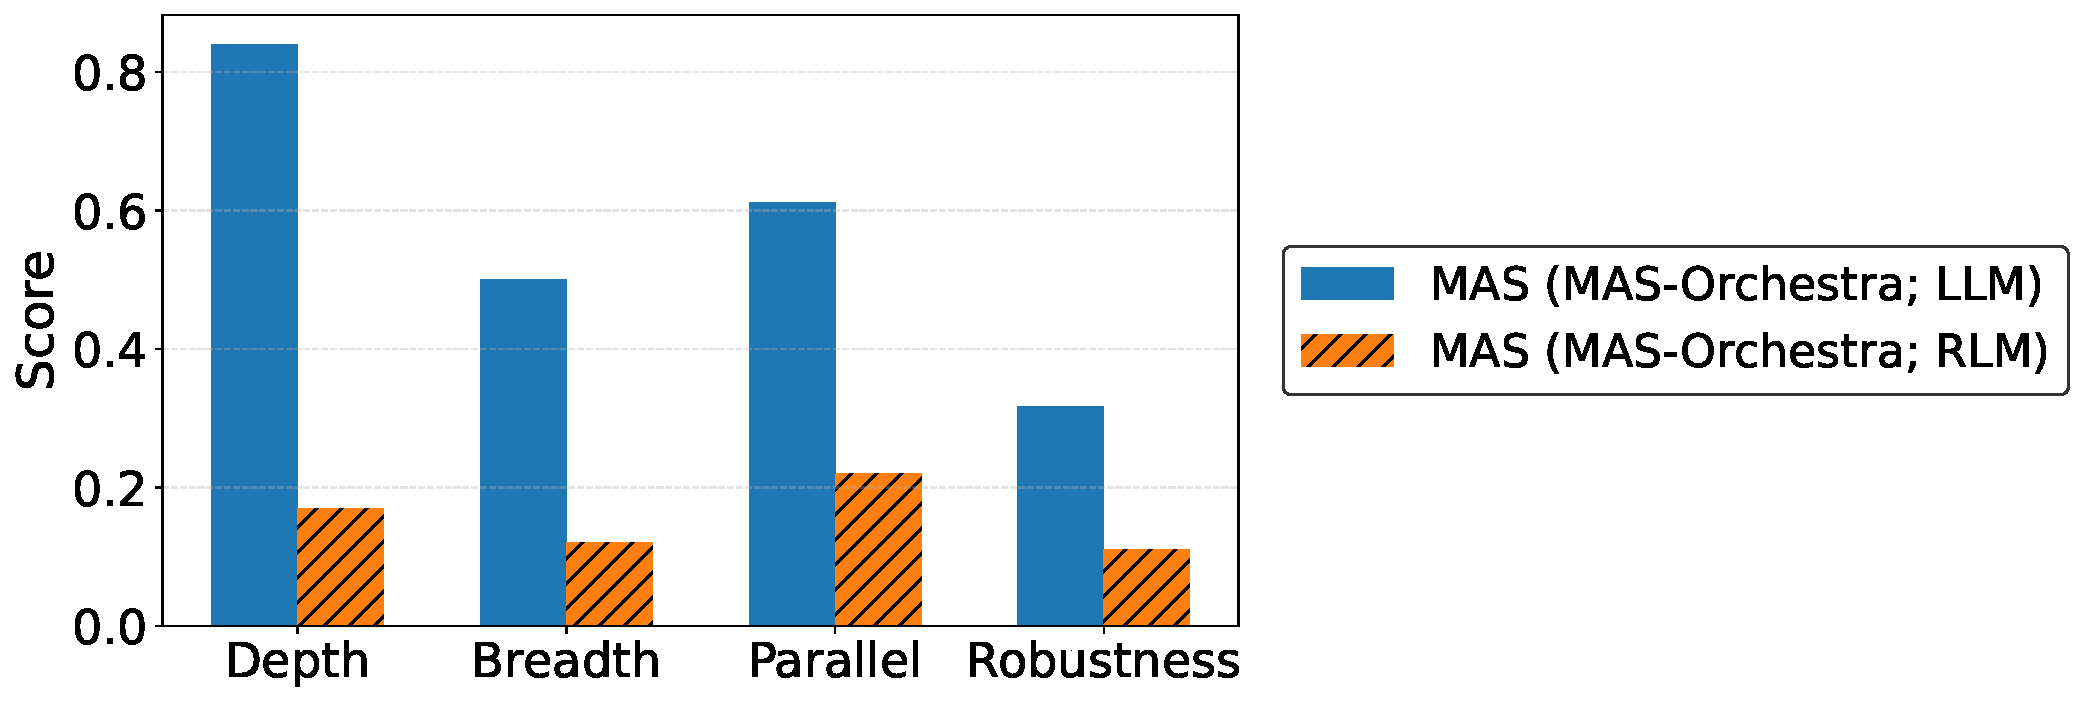
\includegraphics[width=0.6\columnwidth]{figs/deepseek.pdf}
% \vspace{-\baselineskip}
\captionof{figure}{\small 使用\textbf{同等规模}的 LLM（\qwen）和 RLM（\deepseekqwen）作为编排器时的 \avgat{8} 对比。}
\label{fig:deepseek}
\end{center}

\subsection{复杂度泛化}
\label{ap:complexity_generalization}

% To facilitate the investigation of  \textit{complexity generalization}, we train the orchestrator on instances with smaller axis values and evaluate on both the training values and higher, held-out axis values in \ourbenchmark. Additional discussion is provided in \cref{ap:complexity_generalization}, and further
 
为研究\textit{复杂度泛化}，我们在维度取值较小的实例上训练编排器，再在 \ourbenchmark 中的训练取值与更高的留出取值上进行评估。具体而言，模型在取值 2 到 8 的\depth{}数据上训练，评估扩展到 12。对于\breadth{}和\myparallel，训练覆盖取值 2 到 4，评估扩展到 8。对于\horizon{}和\robustness，训练取值范围为 2 到 6，评估最高扩展到 8。

随着任务变得更加复杂，性能会下降。重要的是，分布外复杂度与分布内复杂度遵循相同趋势。这表明 \ourframework 能够受控地提高任务复杂度，并在复杂度增长时表现出一致的泛化行为。
% \zixuan{can move to appendix}



\subsection{以 LLM 与 RLM 作为编排器}
\label{ap:rlm_orchestrator}


\textbf{智能体统计。}\cref{fig:7b_120b_vs_20b_120b_depth4}展示了 MAS-Orchestra 所提出 MAS 中的智能体统计。详细描述与观察见\cref{sec:reasoning_meta_agent}。

\begin{center}
\vspace{-0.5\baselineskip}
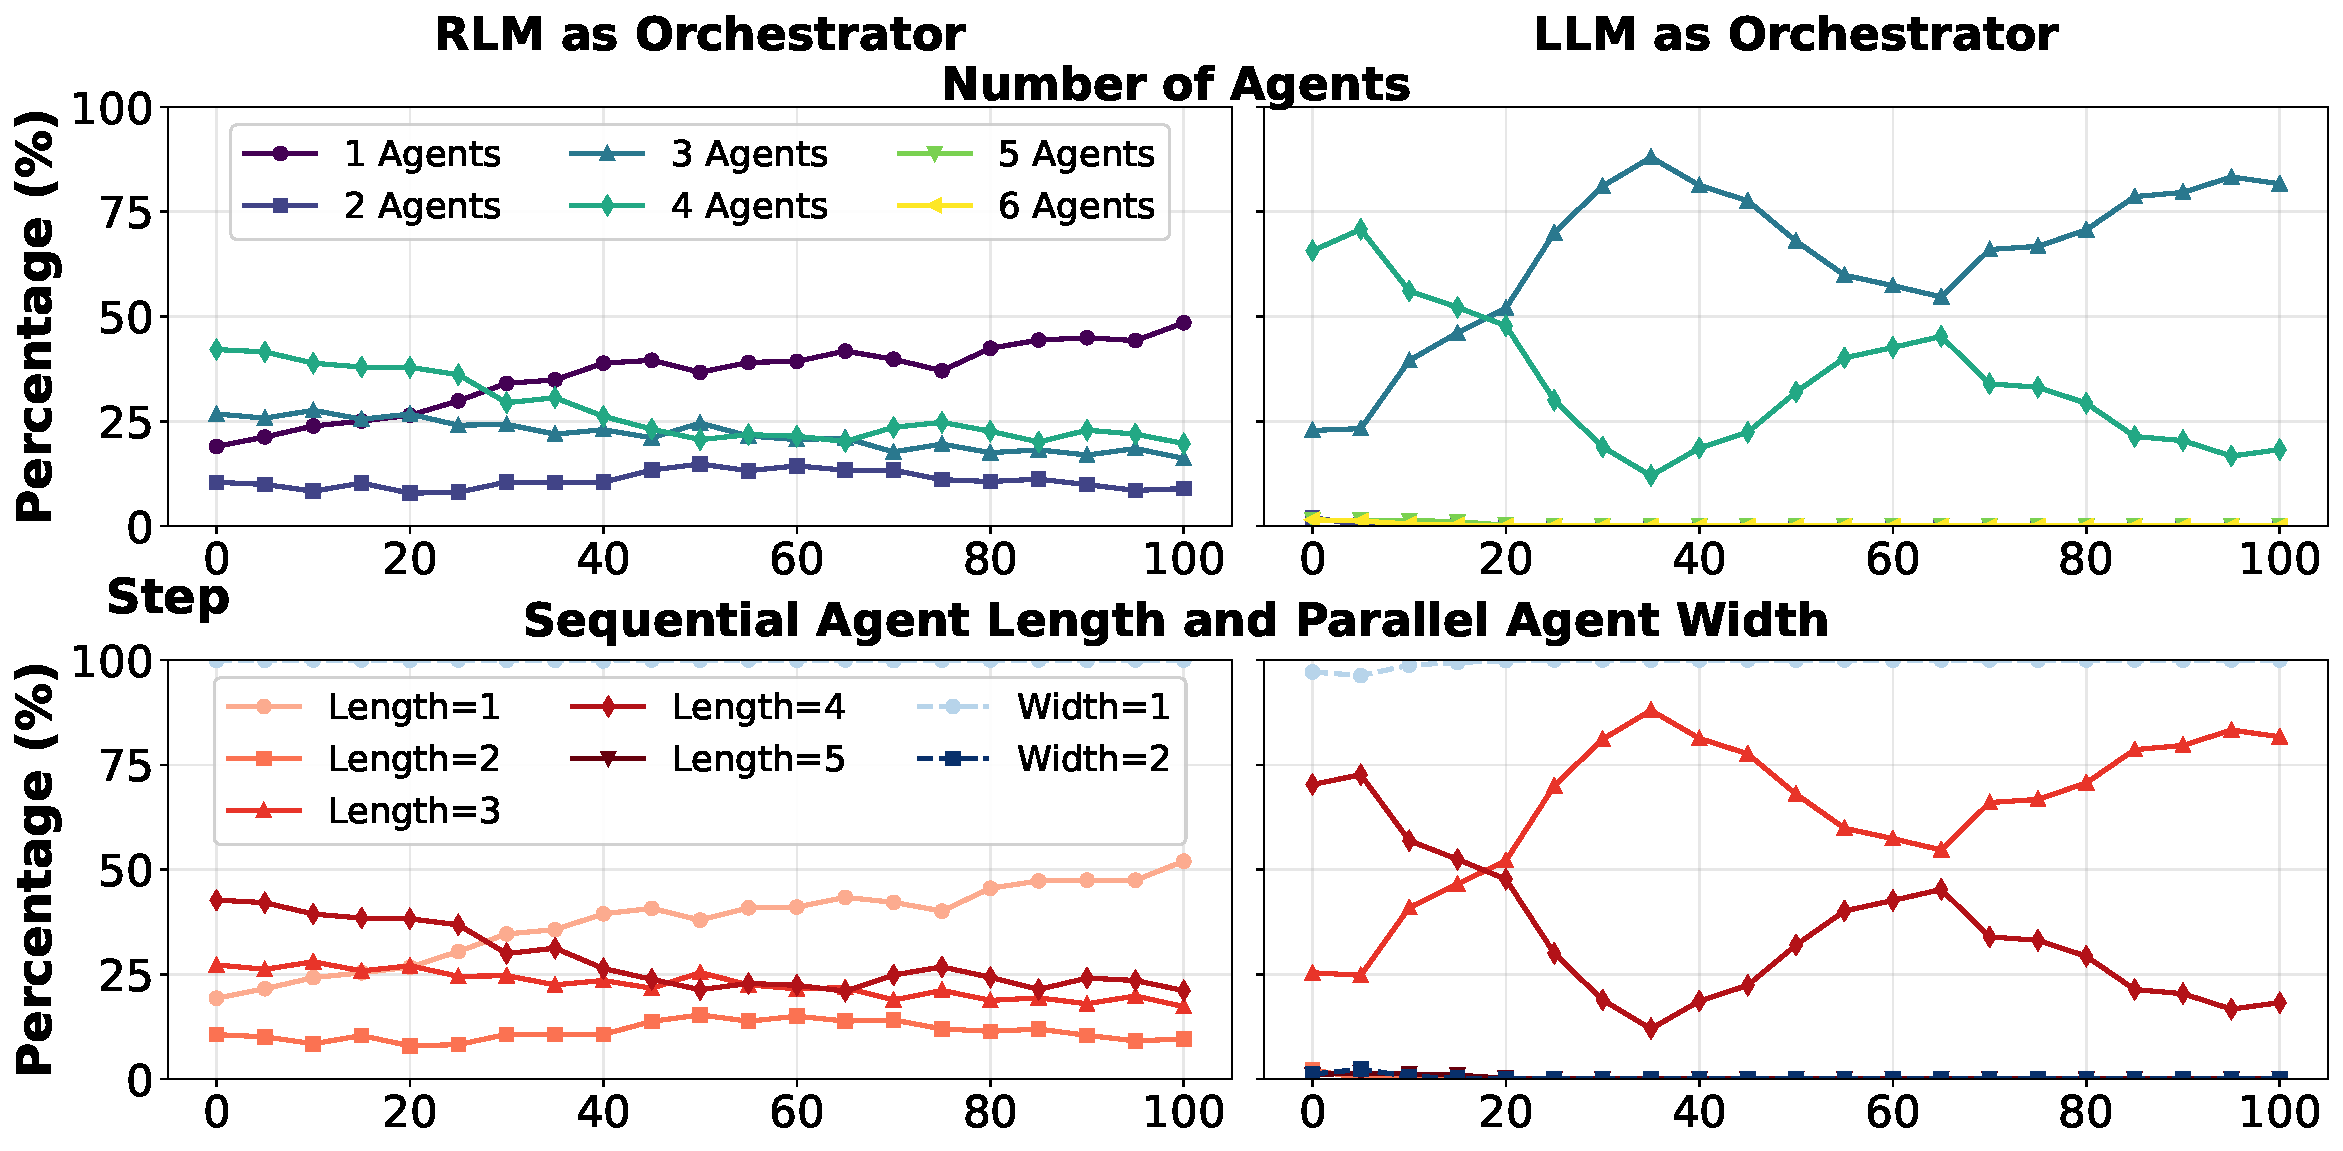
\includegraphics[width=0.8\columnwidth]{figs/7b_120b_vs_20b_120b_depth4.pdf}
% \vspace{-\baselineskip}
\captionof{figure}{\small 训练过程中生成 MAS 的智能体统计（以 \depth 等于 4 为例）。\textit{智能体数量}衡量子智能体总数，\textit{顺序智能体长度}衡量依赖链长度，\textit{并行智能体宽度}衡量子智能体入度。}
\label{fig:7b_120b_vs_20b_120b_depth4}
\end{center}




\textbf{示例。}
在\cref{tab:rlm_example}中，我们展示了一个来自\depth{}维度（\depth{}等于 4）的样本，其中编排器为 \qwen，子智能体为 \ossonetwenty。详细描述与观察见\cref{sec:reasoning_meta_agent}。


% \zixuan{if it is not compare, we may not use table, or add compare,s horten tables}
% \zixuan{consider long table}
\begin{table*}[h!]
\centering
\small
% \addtolength{\tabcolsep}{-0.4em}
\begin{tabularx}{\textwidth}{l X X}
\toprule
\textbf{编排器} & \textbf{\osstwenty} & \textbf{\qwen}\\
\midrule
\textbf{问题} & \multicolumn{2}{p{0.76\linewidth}}{
每个旧金山金门公园食蚁兽的数量等于 21。每个巴黎布洛涅森林袋鼠的数量等于每个墨西哥城查普尔特佩克公园狼的数量。每个巴黎布洛涅森林狼的数量等于 6。……墨西哥城查普尔特佩克公园有多少只驼鹿？}\\
\midrule
\textbf{思考过程} &
分析：我们需要设计智能体。问题是求墨西哥城查普尔特佩克公园的驼鹿数量。先快速解析。

变量定义如下：

GGP\_SF\_Anteater = 21（已知）
GGP\_SF\_Wolf = 12
GGP\_SF\_Moose = ?
GGP\_SF\_Kangaroo = ?
GGP\_SF\_Moose 等于每个墨西哥城查普尔特佩克公园的狼。因此 GGP\_SF\_Moose = CP\_MX\_Wolf。

...

没有其他约束涉及 CP\_MX\_Creatures，因此不存在问题。

因此答案为 42。

可以只创建一个智能体吗？单个智能体能够求解，但我们或许希望使用多智能体展示推理。不过约束允许单智能体，也可以为演示采用多智能体。

更简单的方案是使用一个输入为空的 CoTAgent 直接求解。这最为简洁，但必须确保得到最终答案。提供一个输入为空的最终智能体即可产生最终答案。

是否需要展示中间步骤？没有必要。

既然可以使用单智能体，那就使用单智能体。

...

开始生成。

最终回答<thinking>
  该问题是一个简单的线性方程组，唯一关心的未知量是墨西哥城查普尔特佩克公园的驼鹿数量。
  所有其他变量要么直接给出，要么可以用已知常数表示。
  单个 CoTAgent 即可解析陈述、实例化变量、执行必要代入，并给出最终数值答案。
  由于不需要中间智能体，该图只包含这一个汇点智能体，它同时也是起始节点。
  & 
  <thinking>
  该问题需要建立并求解一个方程组。使用单个智能体并不充分，因为它会混合问题解析与求解步骤，增加出错风险。我们需要先把问题解析为方程，再求解方程组，最后验证解。这样的分工能保证准确性，并允许独立验证每一步。
  最终答案将由 Final\_Answer 智能体给出。
\\
\midrule
\textbf{执行输出} &
21
&
19
\\
\midrule
\textbf{真实答案} & \multicolumn{2}{c}{
19}
\\
\bottomrule
\end{tabularx}
\caption{指令微调 LLM（\qwen）与 RLM（\osstwenty）在同一问题实例上的对比。
% \osstwenty as orchestrator run on one problem instance, including the model output and the ground truth answer.
}
% from https://vincent950129.github.io/mas-design/mas_r1/qwen2.5_20b_oss_120b_low_depth4.html
\label{tab:rlm_example}
\end{table*}



\subsection{更长上下文下高推理强度的\robustness}


\begin{center}
\vspace{-0.5\baselineskip}
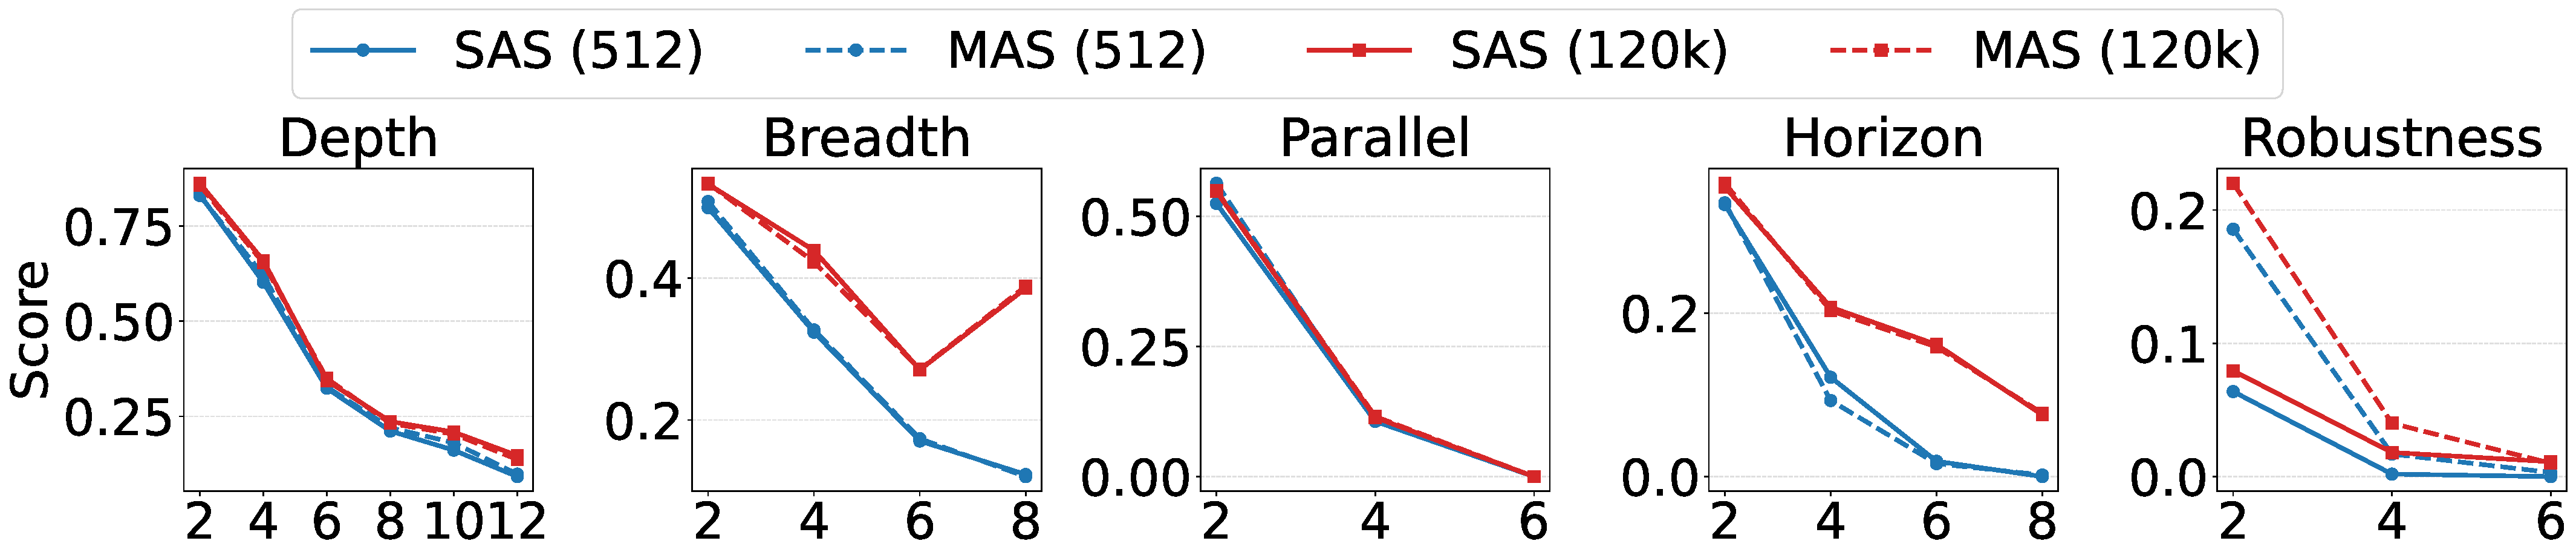
\includegraphics[width=\columnwidth]{figs/max_length.pdf}
\vspace{-\baselineskip}
\captionof{figure}{\small 不同最大上下文长度下的 \avgat{8} 对比，其中编排器为 \qwen，子智能体为 \ossonetwenty。}
\label{fig:max_length}
\end{center}
